\documentclass[12pt,a4paper,oneside]{article}

\usepackage[utf8]{inputenc}
\usepackage[portuguese]{babel}
\usepackage[T1]{fontenc}
\usepackage{amsmath}
\usepackage{amsfonts}
\usepackage{amssymb}
\usepackage{graphicx}
\usepackage{xcolor}
\usepackage{multicol}
% Definindo novas cores
\definecolor{verde}{rgb}{0.25,0.5,0.35}

\author{\\Universidade Federal de Jataí (UFJ)\\Bacharelado em Ciência da Computação \\Linguagens Formais e Autômatos \\Esdras Lins Bispo Jr.}

\date{30 de novembro de 2018}

\title{\sc \huge Prova (Parte 1)}

\begin{document}

\maketitle

{\bf ORIENTAÇÕES PARA A RESOLUÇÃO}

\small
 
\begin{itemize}
	\item A avaliação é individual, sem consulta;
	\item A pontuação máxima desta avaliação é 10,0 (dez) pontos, sendo uma das 06 (seis) componentes que formarão a média final da disciplina: quatro mini-testes (MT), uma prova final (PF), exercícios-bônus (EB) e exercícios aplicados em sala de aula pelo método de Instrução pelos Colegas (IpC);
	\item A média final ($MF$) será calculada assim como se segue
	\begin{eqnarray}
		MF & = & MIN(10, S) \nonumber \\
		S & = & [(\sum_{i=1}^{4} max(MT_i, SMT_i ) + PF].0,2  + EB + IpC\nonumber
	\end{eqnarray}
	em que 
	\begin{itemize}
		\item $S$ é o somatório da pontuação de todas as avaliações, e
		\item $SMT_i$ é a substitutiva do mini-teste $i$.
	\end{itemize}
	\item O conteúdo exigido desta avaliação compreende o seguinte ponto apresentado no Plano de Ensino da disciplina: (1) Revisão de Fundamentos e (2) Autômatos Finitos Determinísticos.
\end{itemize}

\begin{center}
	\fbox{\large Nome: \hspace{10cm}}
\end{center}

\newpage

\begin{enumerate}
	
	\section*{Mini-Teste 1}
	
	\item (5,0 pt) {\bf [Sipser 0.8]} Considere o grafo não-direcionado $G = (V, E)$ em que $V$ , o conjunto de nós, é $\{1, 2, 3, 4\}$ e $E$, o conjunto de arestas, é $\{\{1, 2\}, \{2, 3\}, \{1, 3\}, \{2, 4\}, \{1, 4\}\}$.
	\begin{enumerate}
		\item (2,0 pt) Desenhe o grafo G. 
		
		\vspace*{0.3cm}
		
		{ \color{blue} {\bf Resposta:}
			
			\begin{center}
				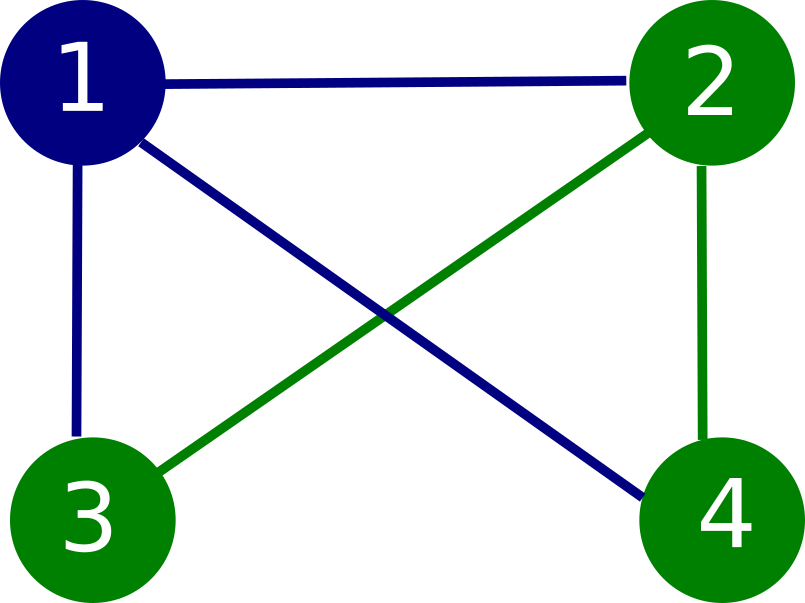
\includegraphics[width=.5\textwidth]{imagens/grafo}
			\end{center}
		
		}
	
		\item (1,5 pt) Qual é o grau do nó 1? E do nó 3?  
		
		\vspace*{0.3cm}
		
		{ \color{blue} {\bf Resposta:} O nó 1 tem grau 3 e o nó 3 tem grau 2.}
		\item (1,5 pt) Indique um caminho do nó 3 ao nó 4 sobre seu desenho de G.
		
		\vspace*{0.3cm}
		
		{ \color{blue} {\bf Resposta:} Indicado de cor {\color{green} \bf verde} na resposta da letra (a).}
	\end{enumerate}
	
	\newpage
	
	\item (5,0 pt) {\bf [IpC - Q022]}
	Um autômato finito é definido por uma 5-upla $(Q, \Sigma, \delta, q_0, F)$. A função $\delta$ é definida como se segue
	\begin{center}
		$\delta:Q \times \Sigma \rightarrow Q$
	\end{center}
	Em relação à $\delta$, marque a alternativa \underline{correta} e \underline{justifique} o motivo das demais serem falsas.

\begin{enumerate}
\item os estados do autômato são necessários apenas no domínio da função.

\vspace*{0.3cm}

{ \color{red} {\bf Resposta:} Não é correto. Não apenas no domínio na função, mas no contradomínio também.}

\item o contradomínio da função é o alfabeto.

\vspace*{0.3cm}

{ \color{red} {\bf Resposta:} Não é correto. O contradomínio da função é o conjunto de estados.}

\item as possibilidades de valores de entradas são infinitas.

\vspace*{0.3cm}

{ \color{red} {\bf Resposta:} Não é correto. $Q$ e $\Sigma$ são finitos. Logo, $Q \times \Sigma$ é finito.}

\item é uma função que recebe duas entradas, sendo um estado e um símbolo do alfabeto.

\vspace*{0.3cm}

{ \color{blue} {\bf Resposta:} Correto.}
\end{enumerate}

\newpage

	\section*{Mini-Teste 2}

	\item (5,0 pt) {\bf [Sipser 1.11]} Prove que todo AFN pode ser convertido em um AFN equivalente que tenha apenas um único estado de aceitação.
	
	\vspace*{0.3cm}
	
	{ \color{blue} {\bf Resposta:} Seja um AFN $N = \{Q, \Sigma \delta, q_0, F\}$. Podemos construir um AFN $O = \{Q', \Sigma' \delta', q_0', F'\}$ que seja equivalente a $N$. Os elementos de $O$ são descritos a seguir:
		\begin{itemize}
			\item $Q' = Q \cup \{q_{novo}\}$;
			\item $\Sigma' = \Sigma$;
			\item $\delta'(q,a) = \left\{\begin{array}{cl}
				\delta(q,a), & \text{se } q \in Q \setminus F\\
				\delta(q,a), & \text{se } q \in F \text{ e } a \not= \epsilon\\
				\delta(q,a) \cup \{ q_{novo} \}, & \text{se } q \in F \text{ e } a = \epsilon\\
				\emptyset	& \text{se } q=q_{novo}\\
				\end{array} \right.$\\
			\item $q_0' = q_0$;
			\item $F' = \{ q_{novo} \}$.
		\end{itemize}
		Logo, todo AFN pode ser convertido em um AFN equivalente que tenha apenas um único estado de aceitação $\blacksquare$.
	}

	\item (5,0 pt) {\bf [IpC - Q037]} Sobre um AFN $M$, marque a alternativa \underline{incorreta} e \underline{justifique} a sua resposta.
\begin{enumerate}
\item para $M$ aceitar $\omega$, é necessário que todos os ramos de execução aceitem $\omega$.

\vspace*{0.3cm}

{ \color{red} {\bf Resposta:} Não é correto. É necessário que pelo menos um dos ramos de execução aceite $\omega$.}

\item a sua função $\delta$ tem como saída um conjunto de estados.

\vspace*{0.3cm}

{ \color{blue} {\bf Resposta:} Correto.}

\item a sua função de $\delta$ tem como uma de suas entradas um símbolo de $\Sigma_{\epsilon}$.

\vspace*{0.3cm}

{ \color{blue} {\bf Resposta:} Correto.}

\item $M$ tem apenas um estado inicial.

\vspace*{0.3cm}

{ \color{blue} {\bf Resposta:} Correto.}

\end{enumerate}

\end{enumerate}

\end{document}